\message{ !name(paper.tex)}%  article.tex (Version 3.3, released 19 January 2008)
%  Article to demonstrate format for SPIE Proceedings
%  Special instructions are included in this file after the
%  symbol %>>>>
%  Numerous commands are commented out, but included to show how
%  to effect various options, e.g., to print page numbers, etc.
%  This LaTeX source file is composed for LaTeX2e.

%  The following commands have been added in the SPIE class 
%  file (spie.cls) and will not be understood in other classes:
%  \supit{}, \authorinfo{}, \skiplinehalf, \keywords{}
%  The bibliography style file is called spiebib.bst, 
%  which replaces the standard style unstr.bst.  

\documentclass[]{spie}  %>>> use for US letter paper
%%\documentclass[a4paper]{spie}  %>>> use this instead for A4 paper
%%\documentclass[nocompress]{spie}  %>>> to avoid compression of citations
%% \addtolength{\voffset}{9mm}   %>>> moves text field down
%% \renewcommand{\baselinestretch}{1.65}   %>>> 1.65 for double spacing, 1.25 for 1.5 spacing 
%  The following command loads a graphics package to include images 
%  in the document. It may be necessary to specify a DVI driver option,
%  e.g., [dvips], but that may be inappropriate for some LaTeX 
%  installations. 
\usepackage{graphicx}
\usepackage{subfig}
\usepackage{amsmath}
\usepackage{amssymb}
\usepackage{hyperref}

\title{Texture mapping 3D planar models of indoor environments with noisy camera poses} 

%>>>> The author is responsible for formatting the 
%  author list and their institutions.  Use  \skiplinehalf 
%  to separate author list from addresses and between each address.
%  The correspondence between each author and his/her address
%  can be indicated with a superscript in italics, 
%  which is easily obtained with \supit{}.

\author{Peter Cheng, Michael Anderson, Stewart He, Avideh Zakhor
\skiplinehalf
University of California, Berkeley\\
}

 

%%%%%%%%%%%%%%%%%%%%%%%%%%%%%%%%%%%%%%%%%%%%%%%%%%%%%%%%%%%%% 
%>>>> uncomment following for page numbers
% \pagestyle{plain}    
%>>>> uncomment following to start page numbering at 301 
%\setcounter{page}{301} 
 
\begin{document}

\message{ !name(paper.tex) !offset(278) }
\subsection{Geometry-based Alignment}
\label{sec:geometryAlignment}
After computing each image's projection onto the target surface, as
described in Section \ref{sec:simpleTextureMapping}, we detect lines
in the projections using Hough transforms. Experience and intuition
show that walls in indoor environments contain linear features that
are either horizontal or vertical, often corresponding to doors,
windows, posters, etc. Thus, when texturing walls, we rotate images in
2D such that dominant lines are made to be horizontal or
vertical. This can be further extrapolated by orienting lines with a
wall's boundaries, for example in areas with a slanted roof.

\begin{figure}
  \centering
  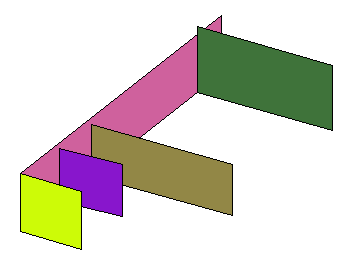
\includegraphics[height=1.5in]{geometryAlign_planes.png}
  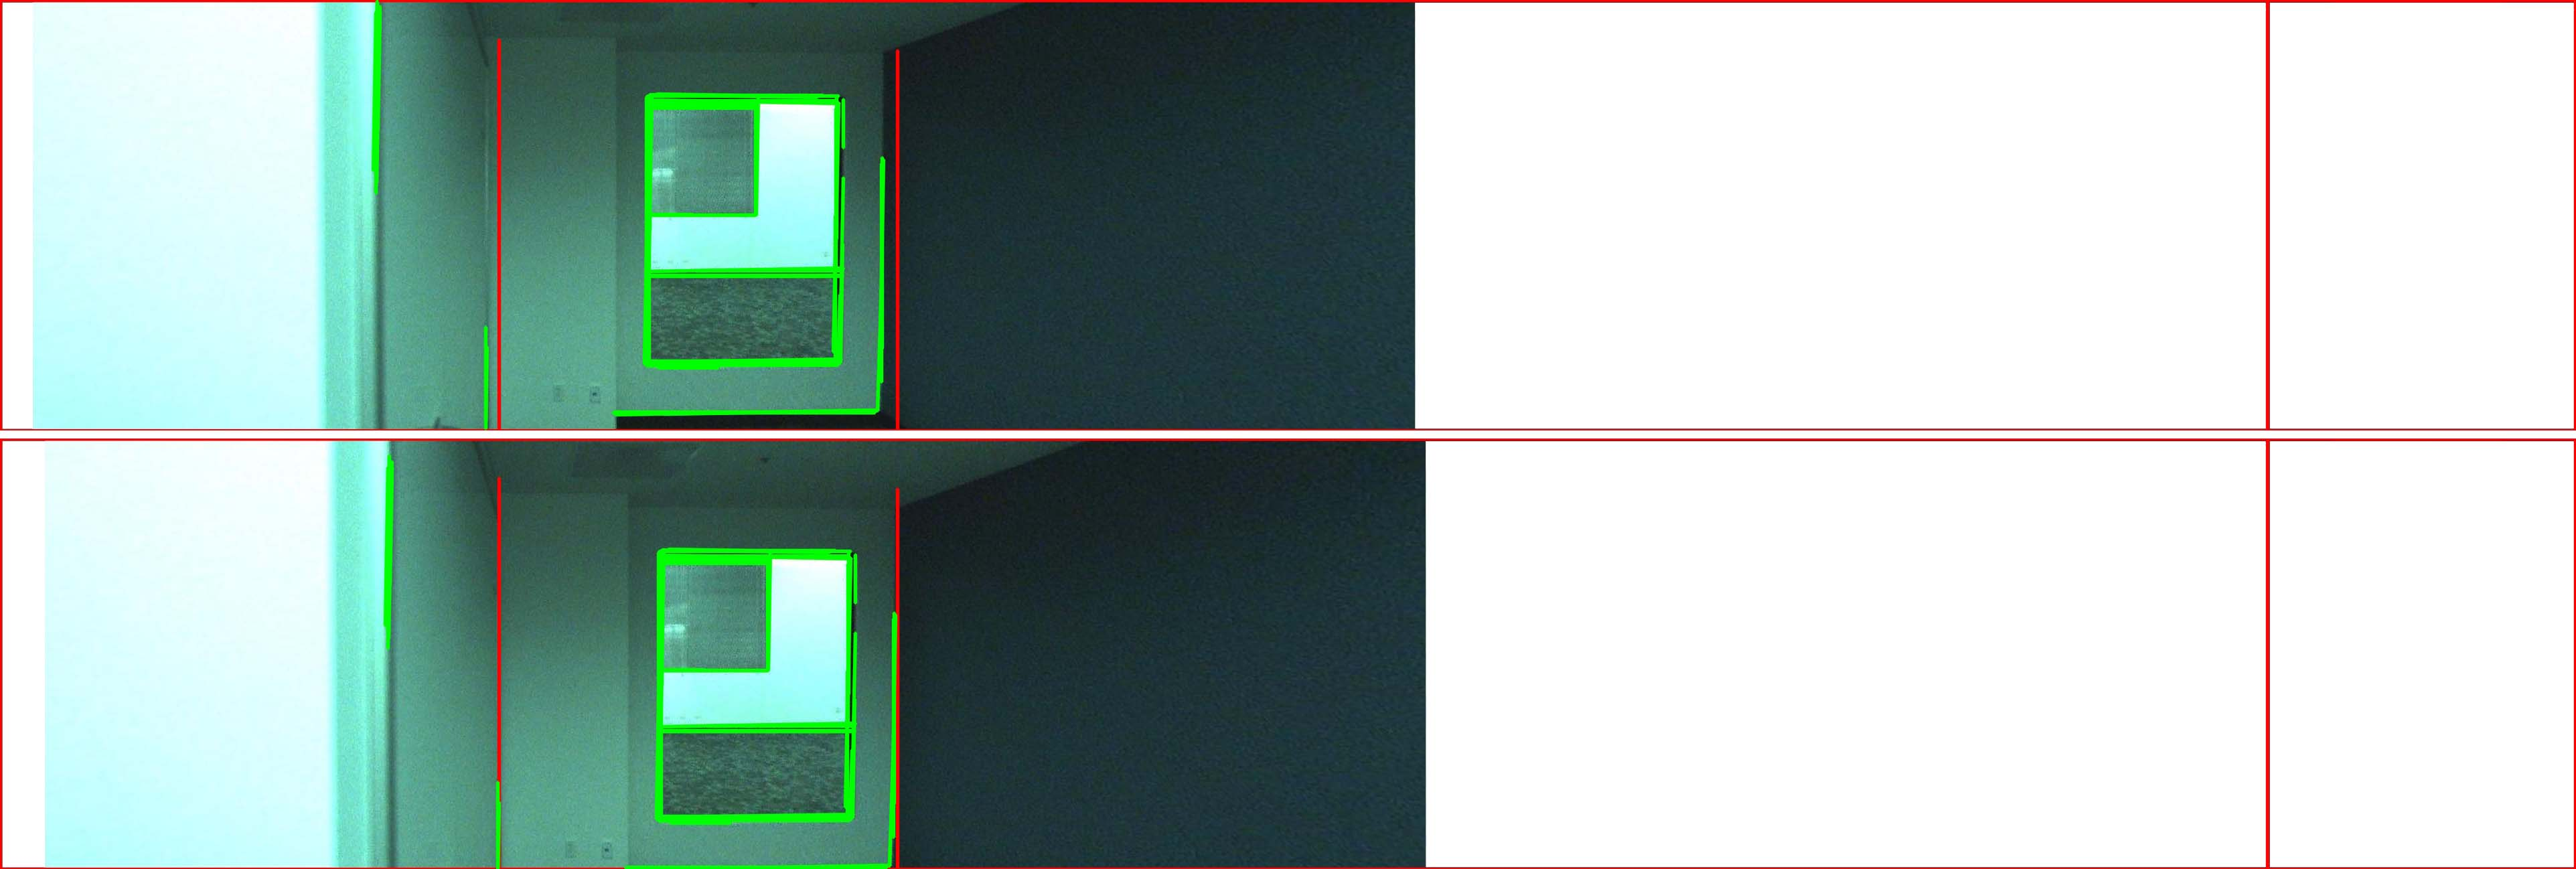
\includegraphics[height=1.5in]{geometryAlignment.jpg}
  \caption{(a) When texturing the red surface, it makes sense to align images to surface boundaries and intersections. (b) Red lines are geometry-based lines, while green lines are detected in the image via Hough transform. Above is the original projection, and below is the image adjusted for alignment.}
  \label{fig:geometryAlignment}
\end{figure}


At this point in time, image occlusions have not been accounted
for. As a result, some image projections contain texture that should
project to an adjacent surface, generally with a linear boundary where
the two surfaces meet. If this linear boundary is detected by Hough
transform, the image is rotated and shifted in 2D such that the visual
boundary between two surfaces matches the physical boundary in our
digital model. An example of such an adjustment is in Figure
\ref{fig:geometryAlignment}

To perform the rotation and alignment, one method would be to detect
all line matches and solve for an optimal homography. In nearly all
cases however, we find that a single 2D rotation is sufficient to
properly align lines in an image. We also rarely have more than one
linear geometry feature to match to in each orthogonal
direction. Thus, for a rotation angle, we simply take all angles
between image-based and geometry-based lines under 5 degrees, and
average them. After the image is rotated, we find the horizontal and
vertical image-based and geometry-based line segments with minimum
orthogonal distance between them. For both distances, if it is under 5
mm, we apply the corresponding shift, and indicate that the image was
aligned to geometry in one or both dimensions, which reduces further
shifting in Section \ref{sec:robustSIFTFeatureMatching}.

\message{ !name(paper.tex) !offset(679) }

\end{document} 
